\section{Model Boid}
Počítačový model pro řízení hejna zvířat jako jsou ptáci a ryby popsal Craig Reynolds v roce 1986. Jednotlivé jedince nazval Boidy. Samotný model pak prezentoval na konferenci SIGGRAPH o rok později. 
\par
Od roku 1987 byl model Boid použit pro velké množství simulovaného chování hejna. Prvním, veřejně známým použitím byl film Batman se vrací (1992) od Tima Burtona. Obsahuje počítačově simulované chování hejna netopýrů a skupiny tučňáků, které bylo vytvořeno upravenou verzí modelu Boid. \cite{ReynoldsBoid}

\subsection{Popis modelu}
Boid pracuje s agenty reprezentovanými pozicí a rychlostním vektorem. Model lze aplikovat pro pohyb ve dvou i třech rozměrech. 
\par
Každý agent se řídí třemi základními pravidly, podle kterých upraví svůj rychlostní vektor každý časový úsek. Jedná se o Separaci, Vyrovnání a Kohezi. 

\newcommand\litem[1]{\item{\bfseries #1,\\}}
\begin{enumerate}
	\litem {Separace}
	Agent se snaží nesrazit s jinými agenty. Upravuje proto svůj směrový vektor, aby se dostal od příliš blízkých agentů. 
	\begin{figure}[H]
		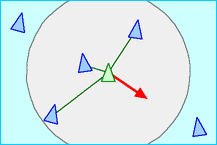
\includegraphics[width=5cm]{separation.png}
		\centering
		\caption{Separace (Separation) \cite{ReynoldsBoid}}
	\end{figure}

	\litem {Vyrovnání}
	Agent se chce pohybovat stejným směrem a rychlostí jako jeho sousedé. Upravuje svůj vektor podle průměru z jeho okolí. 
	\begin{figure}[H]
		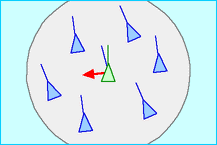
\includegraphics[width=5cm]{alignment.png}
		\centering
		\caption{Vyrovnání (Alignment) \cite{ReynoldsBoid}}
	\end{figure}

	\litem {Koheze}
	Agent upravuje svůj rychlostnní vektor tak, aby se dostal do pomyslného středu všech sousedních agentů. 
	\begin{figure}[H]
		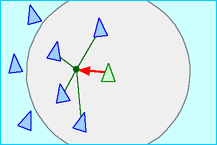
\includegraphics[width=5cm]{cohesion.png}
		\centering
		\caption{Koheze (Cohesion) \cite{ReynoldsBoid}}
	\end{figure}
\end{enumerate}
Každý boid má přímý přístup ke všem objektům ve scéně, nicméně tento model vyžaduje, aby reagoval pouze na své okolí. To je definováno maximální vzdáleností a zorným úhlem agenta. Můžeme přidávat i další pravidla jako třeba minimální vzdálenost nebo úhel mezi dvěmi agenty apod. Pravidla, podle kterého jedinec rozlišuje okolí, si můžeme představit jako smysly daného zvířete.  
\begin{figure}[H]
	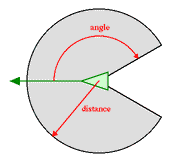
\includegraphics[width=5cm]{neighborhood.png}
	\centering
	\caption{Okolí agenta \cite{ReynoldsBoid}}
\end{figure}

Jak bylo na začátku kapitoly naznačeno, model můžeme různě zozšiřovat. Sám Reynolds přišel rok po představení svého modelu na stejné koferenci s rozšířením pro výhýbání se překážkám. Detailněji vše vysvětluje ve své práci Not bumping into things \cite{ReynoldsBoidNoBump}. V podstatě se jedná o úpravu výsledného vektoru rychlosti pokud se před jedincem nachází nějaký objekt. 
\par
Pokud jednotlivým pravidlům přiřadíme váhy, můžeme následnými úpravami těchto vah měnit chování konkrétního jedince či celého hejna. Boidi tak můžou uzpůsobovat své chování v závislosti na prostředí. Například je-li v okolí dravec, budou mít mezi sebou větší rozestup, hlídat si větší okolí, rychleji reagovat na změnu směru atd. 